\documentclass{article}
\usepackage{graphicx} % Required for inserting images
\usepackage{geometry}
 \geometry{
 a4paper,
 total={170mm,257mm},
 left=20mm,
 top=20mm,
 }
\graphicspath{{../results/}}

\title{\huge Is Florida getting warmer?}
\author{Tianle Shao}
\date{November 2023}

\begin{document}

\maketitle

\section{Introduction}

This investigation makes use of temperature data from Key West (Florida, USA) over a period of 100 years from 1901 to 2000, to determine if temperature has increased significantly within this period.

\section{Methods}

The correlation between years and temperatures of Florida was found using Spearman's rank correlation coefficient (rho). To see if the temperature of Florida has increased, a permutation anaylsis was used, where the rho value calculated was compared to that of random samples. The year-temperatures pairs for the original Florida dataset were randomised 10,000 times, and the corresponding rho values compared with that of the original Florida dataset.

\begin{figure}[h]
    \centering{}
    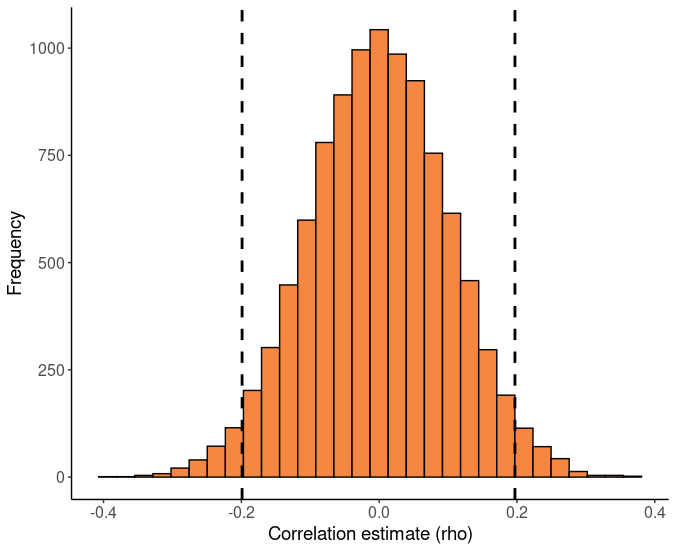
\includegraphics[width=0.5\textwidth]{Florida_Histogram.png}
    \caption{The distribution of rho values from 10,000 random repeats.}
    \label{fig:Histogram}
\end{figure}

\section{Results \& Interpretation}

The Spearman's rank correlation coefficient (rho) was 0.526 for the correlation between years and temperatures of Florida. This was found to be higher than 100\% of the 10,000 randomly generated rho values, corresponding to a P-value of 0. This suggests that the average temperature of Florida has increased significantly over the period from 1901 to 2000.

\end{document}
